\section{Transitivity}
For the map $f:\;X \to X$, where $f$ acts as Eq.(\ref{eq:themapf})

\begin{equation}
    \label{eq:themapf}
    f^{n+1}(x)=\mu f^n(x) \times (1-f^n(x))
\end{equation}

,transitivity means that
for the domain $X$ defined by Eq.(\ref{eq:domain}),

\begin{equation}
    \label{eq:domain}
    \{x \in \mathbb{R} \; \mid \;  0 \leq x \leq 1 \}
\end{equation}

there are some finite number of iterations $n$ that would
produce a result in the co-domain $X$ defined as Eq.(\ref{eq:domain})
,illustrated in Fig.\ref{fig:setnime}.

\begin{figure}[h]
    \centering
    \includegraphics[width=0.4\textwidth]{Images/setnime.png}
    \caption{Visualisation of $f:\;X \to X$}
    \label{fig:setnime}
\end{figure}

This implies that where $f$ behaves chaotically it will \textbf{not} converge
towards one or multiple values, but rather take up all points within 
a set. In Fig.\ref{fig:trans1} we observe how many unique values $f$ generates against $\mu$,
where $\mu$ is the Growth Rate as expressed in Eq.(\ref{eq:themapf}).

\begin{figure}[h]
    \centering
    \includegraphics[width=0.8\textwidth]{Images/trans 1.png}
    \caption{Unique values of $f$ to 5 decimal places against $\mu$ }
    \label{fig:trans1}
\end{figure}

Before counting the unique values the map generates, we let the system stabilize
running it over 2'000'000 iterations without recording anything. Then values unique to 
5 decimal places are recorded. For $0\leq \mu < 3$, $f$ converges to a single value,
then at equal intervals we observe doubling. The system converges to 2, 4, 8, 16, 32, ...,
unique values.

\begin{figure}[h]
    \centering
    \includegraphics[width=0.8\textwidth]{Images/Untitled.png}
    \caption{Unique values of $f$ to 5 decimal places against $\mu$}
    \label{fig:trans2}
\end{figure}

As we look at further values of $\mu$ (Fig.\ref{fig:trans2}), this pattern is broken.
We stop observing doubling, rather $f$ begins generating a very large amount of unique
values. When we begin recording values, we run the map over 50'000 iterations.
Out of those, for $\mu > 3.695$, approximately 40'000 are unique to 5 decimal places.
This hints that at that Growth Rate $f$ becomes Transitive, generating unique values 
and allowing for any value in the co-domain to be reached allowing enough iterations. Sec.~\ref{appendix:transitivity}\\
The exact value of $\mu$ at which Eq.(\ref{eq:themapf}) becomes Transitive is

\begin{equation}
    3.570 \pm 0.005
\end{equation}


%------------------------------------------------------------------------
\newpage
\section{Dense in $X$}
For our map - Eq.(\ref{eq:themapf}), to be Dense in $X$, means that all points
the map $f$ can generate, regardless of the number of iterations, belong to
the domain of $X$ as defined in Eq.(\ref{eq:domain}).

While Transitivity and Sensitivity to Initial Conditions generally become
true where the map $f$ is chaotic (not surprising, as we are using them as
definitions of what being chaotic is), to be Dense in $X$ is a more of a formality.
The system being Dense in the co-domain is not a good sign of whether $f$ is
chaotic or not. It simply means that the system behaves. For $\mu \in [0,\; 4]$,
$f^n (x)$ will always produce a result in the domain, regardless of how many
iterations $n$ it undergoes \cite{baker} .\\

\begin{figure}[h]
    \centering
    \includegraphics[width=0.5\textwidth]{Images/max at 0.png}
    \caption{Plot of $f^n(x)$ versus $x$ for $\mu \in [0,\; 4]$}
    \label{fig:topof0}
\end{figure}

Looking at Fig.(\ref{fig:topof0}) Sec.~\ref{appendix:maxvalue} we can conclude that Max.($f^n(x)$) lies at

\begin{equation}
    \frac{\partial (f^n(x))}{\partial x}\; = \mu (1 - 2x) = 0 
\end{equation}

Thus Max.($f^n(x)$) resides at $x = 0.5$ for all $\mu$. Using this we can rigorously redefine the domain of $\mu$.
$f^n(x) \in [0,\; 1]$; Max.($f^n(x)$) = 1. 

\begin{equation}
    MAX\,(f^n(x)) = \mu 0.5 (1 - 0.5) = \frac{\mu}{4} = 1
\end{equation}
    


Therefore $\mu = 4$ is the higher boundary, and because negative values are undesirable
$\mu = 0$ is the lower boundary.

% The author leaves this proof for 
%the more mathematically inclined readers.\\
What is important is that outside of the scope of $\mu$ defined above, the system misbehaves
generating negative values or tending to infinity. There are different maps
with similar properties, where $\mu$ belongs to a different range. For 
Eq.(\ref{eq:themapf}) we will only work with $\mu \in [0,\; 4]$, as those are the values
where chaos is possible.





%------------------------------------------------------------------------
\section{Sensitivity to Initial Conditions}
\subsection{The Lyapunov Exponent}

The Lyapunov exponent is a measure of divergence between two 
systems, $f(x)$ and $f(x+\Delta x)$, evolving from slightly 
different initial conditions. This divergence is defined to be:

\begin{equation}
\label{eq:2.1}
    f^n (x+\Delta x) - f^n (x) \approx \Delta x\, e^{\lambda n}
\end{equation}

where $n$ is the $n^{th}$ iterate - $f^n (x)$,\\ 
$\lambda$ is the Lyapunov exponent and represents the average 
rate of divergence.\\
If $\lambda$ is negative, $f^n (x)$ and $f^n (x+\Delta x)$ 
converge as $n \to \infty$.\\
If $\lambda$ is positive 
$f^n (x)$ and $f^n (x+\Delta x)$ diverge; the system 
is sensitive to initial conditions \cite{baker}.\\
To be able to enumerate $\lambda$ in later computations 
Eq.(\eqref{eq:2.1}) is rearranged as shown below.\\
Eq.(\eqref{eq:2.1}) can be written as:

\begin{equation}
    \label{eq:2.2}
    \lambda \approx \frac{1}{n} ln \left[ \frac{f^n (x+\Delta x) - f^n (x)}{\Delta x} \right] 
\end{equation}

as $\Delta x \to 0$, this equation takes the form

\begin{equation}
    \lambda \approx \frac{1}{n} ln\left| \frac{d(f^n (x))}{d x} \right| 
\end{equation}
 


Applying the chain rule to the derivative of 
the $n^{th}$ iteration and taking the limit of $n \to \infty$ gives:

\begin{equation}
    \label{eq:2.3}
    \lambda = \lim_{n\to\infty} \frac{1}{n} \sum_{i=0}^{n-1} ln|f'(x_i)|
\end{equation}
%------------------------------------------------------------------------
\subsection{Methodology and the Code}
\label{section:MethodologyAndCode}
Throughout this paper there will be several sections 
discussing the technicalities of the code used to generate
the data and graphs used in the writing of this work.
The reader should not feel obliged to read through this in detail
as the rest of the discussion will repeat any necessary information.
This section is meant for those with interest in the exact workings
of the software.
\paragraph{}
While \eqref{eq:2.3} is certainly a more mathematically rigorous 
definition of the Lyapunov exponent, \eqref{eq:2.2} has its 
"derivative" part of the equation expressed in a more code friendly
way and ultimately the equation used to obtain the Lyapunov exponent
becomes:

\begin{equation}
    \label{eq:2.4}
    \lambda = \lim_{n\to\infty} \frac{1}{n} \sum_{i=0}^{n-1} ln\left| \frac{f^n (x_i+\Delta x) - f^n (x_i)}{\Delta x} \right| 
\end{equation}

\begin{lstlisting}[language=Python, caption=Lyapunov\_Exponent.py excerpt]
def lyapunov(rate):
    """Returns Lyapunov exponent for rate over N gen."""
    function = 0.2
    g_function = function+DX
    lambda = 0

    for i in range(N):
        function = rate * function * (1 - function)
        g_function = rate * d_function * (1-g_function)

        if g_function-function == 0:
            break

        lambda += d.Decimal(abs(g_function - function) / DX).ln()

    lambda = lambda / (i + 2)
    return lambda
\end{lstlisting}

The \textbf{lyapunov} function (as seen in Listing 2.1) begins by defining two variables:

\begin{equation}
    f^0(x)=0.2\; \; \; \; \; \; ;\;f^{n+1}(x)=\mu f^n(x) \times (1-f^n(x))
\end{equation}
    
\begin{equation}
    g^0(x)=f^0(x) + \Delta x \; \; \; \; \; \; ;\;g^{n+1}(x)=\mu g^n(x) \times (1-g^n(x))
\end{equation}



\eqref{eq:2.4} Defines $\lambda$ with a limit $n \to \infty$, unfortunately
that is impractical. Rather than asking \textbf{Is it possible to generate
an infinite number of iterations?}, we should ask \textbf{When is it reasonable
to stop?}\\
To answer this question lets look at where we \textbf{have} to stop.
The standard \textit{float} has 16 decimals of precision. Importing the
\textsc{decimal} module allows pushing that to 26. Pushing that even further,
although possible, would heavily impact processing time and is therefore not 
an option for this project. Even so, if the two systems are identical up to the 
26th digit after \textbf{n} iterations, it is safe to say that they do not
exhibit sensitivity to initial conditions and are therefore not chaotic.\\
To form an idea of how many iterations it is reasonable to run (Listing 2.1) for,
we look at Fig.\ref{fig:fig1}.
\begin{figure}[h]
    \centering
    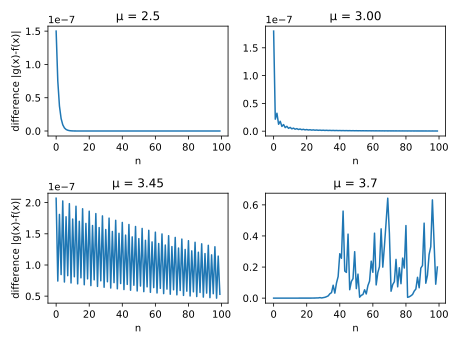
\includegraphics[width=0.8\textwidth]{Images/difference.png}
    \caption{Difference $g^n(x)-f^n(x)$ after n-th iteration.}
    \label{fig:fig1}
\end{figure}

The values for $\mu$ specify the rate of growth in $f^{n+1}(x)=\mu f^n(x) \times (1-f^n(x))$.
The paper covers these in detail later. As for now the reader needs to know that:\\
For $0<\mu<1$, $\; \;f^{n+1}(x)\;\to\;0$ as $n\to \infty$,\\
for $1<\mu<3$, $\; \;f^{n+1}(x)\;\to\;$const. as $n\to \infty,$\\
for $3<\mu<3.57$, $\; \;f^{n+1}(x)$ oscillates between several values\\
for $\approx 3.57<\mu<4$, $\; \;f^{n+1}(x)$ becomes chaotic.
\paragraph{}
Taking another look at Fig.\ref{fig:fig1}. At low values of growth -$\mu$,
it is clear that 20 iterations is enough for the two systems to become nearly identical 
up to the 26th digit. Where the systems oscillate between values, their difference 
slowly tends towards 0, which is more obvious in Fig.\ref{fig:fig2}. 2000 iterations
are not needed however, as even after 40 the difference between the two systems
is of the order $10^{-7}$, which is sufficient to declare them as not sensitive to
initial conditions.

\begin{figure}[h]
    \centering
    \includegraphics[width=0.7\textwidth]{Images/diff3.45555.png}
    \caption{Difference $g^n(x)-f^n(x)$ after n-th iteration at rate of growth $\mu=3.45$. The two systems oscillate between 4 values.}
    \label{fig:fig2}
\end{figure}

With chaotic systems, interesting behaviour occurs after the 40th 
iteration exerting the same behaviour to infinity. As such
the author finds that iterations over \textbf{n=100} are wasteful
in time, although some figures are generated with \textbf{n=1000},
where higher precision is needed.
Equipped with this knowledge we look at (Listing 2.1) again. 
Iterating $g^n(x)$ and $f^n(x)$ n=100 times, it effectively solves the equation:

\begin{equation}
    \label{eq:2.5}
    \lambda = \frac{1}{100} \sum_{i=0}^{99} ln\left| \frac{f^n (x_i+\Delta x) - f^n (x_i)}{\Delta x} \right| 
\end{equation}

Unless the difference $g^n(x)-f^n(x) = 0$, in which case it breaks the execution and solves \ref{eq:2.5}
for however many times the \textbf{for} cycle was iterated. The \textbf{lyapunov} function then returns $\lambda$ and maps it
to the corresponding rate ($\mu$) value that it was solved for. The process then start all over again,
performing the same operations for a slightly larger rate ($\mu$). In the code as seen at \ref{appendix:lyapunov}
the difference between one $\mu$ and the one for which the \textbf{lyapunov} function will be solved
thereafter is called \textsc{resolution}.

\newpage
\subsection{Lyapunov Exponent Graph and Sensitivity to Initial Conditions}

\begin{figure}[h]
    \centering
    \includegraphics[width=0.7\textwidth]{Images/Lyapunov 3.1.png}
    \caption{Lyapunov Exponent $\lambda$ as a function of the Growth Rate $\mu$ 
    for the logistic map$f^{n+1}(x)=\mu f^n(x) \times (1-f^n(x))$, 
    where $\mu \in [3,4]$. \textbf{Positive} $\lambda$ values signify
    sensitivity to initial conditions.}
    \label{fig:fig3}
\end{figure}

As discussed in \ref{section:MethodologyAndCode} \textbf{Methodology and the Code},
the Lyapunov Exponent has been solved for the logistic map 

\begin{equation}
    \label{eq:2.6}
    f^{n+1}(x)=\mu f^n(x) \times (1-f^n(x))
\end{equation}

The key variable in this equation is $\mu$. It is also referred to as the Growth Rate element,
as it controls how $f^{n+1}(x)$ grows in comparison to $f^n(x)$.\\
For $0<\mu<1$, $\; \;f^{n+1}(x)\;\to\;0$ as $n\to \infty$,\\
for $1<\mu<3$, $\; \;f^{n+1}(x)\;\to\;$const. as $n\to \infty,$\\
for $3<\mu<3.56$, $\; \;f^{n+1}(x)$ oscillates between several values\\
for $3.56<\mu<4$, $\; \;f^{n+1}(x)$ becomes chaotic.
\paragraph{}
Fig.\ref{fig:fig3} shows the Lyapunov exponent for $\mu \in [3,4]$ as that is
where the system behaves dynamically (does not settle on one value over time) 
and is of interest to us. The first thing one notices is that even where the 
system is dynamical it is not necessarily chaotic. The reason for this is
reviewed in detail in \ref{section:understandingChaos} \textbf{Towards an 
Understanding of Chaos}. $\lambda$ becomes positive for the first time at
\textbf{3.56986} as seen in fig.\ref{fig:fig4}.

\newpage
\begin{figure}[h]
    \centering
    \includegraphics[width=0.7\textwidth]{Images/Lyapunov 3.3.1.png}
    \caption{Close up of fig.\ref{fig:fig3}. Lyapunov Exponent $\lambda$ becomes positive at $\mu = 3.56986$}
    \label{fig:fig4}
\end{figure}


Obtaining the uncertainty in this value is not
a straightforward process. Traditionally uncertainty would be obtained as:


\begin{equation}
    \label{eq:2.7}
    \lambda = \frac{1}{n} \sum_{i=0}^{99} ln\left| \frac{g^n (x_i) - f^n (x_i)}{\Delta x} \right|
\end{equation}

Where, like in \ref{section:MethodologyAndCode} \textbf{Methodology and the Code}, $f^n (x_i+\Delta x) = g^n (x)$.

\begin{equation}
    \label{eq:2.8}
    d\lambda = \sqrt{ \left( \frac{d\lambda}{dg} \Delta g \right)^2 +\left(\frac{d\lambda}{df} \Delta f \right)^2} =
    \frac{1}{100} \sum_{i=0}^{99} \frac{1}{g^n (x_i) - f^n (x_i)}
\end{equation}

In this case $\Delta g$ and $\Delta f$ would be the limits of accuracy touched on in \ref{section:MethodologyAndCode},
which are 26 digits of accuracy. If one were to solve the above equation he would obtain $d\lambda \approx 10^{-21}$.
Unfortunately this is not the case. Error arises long before the program runs out of digits to store data in.
Manipulating $\Delta x$ (in $f^n (x+\Delta x)$) results in significant changes, as seen in fig.~\ref{fig:fig5}. 

\begin{figure}[h]
    \centering
    \includegraphics[width=0.7\textwidth]{Images/Lyapunov 5O.png}
    \caption{Variations of fig.\ref{fig:fig3} with different values for $\Delta x$.
    \textbf{A)}$\Delta x = 10^{-3}$, Chaos onset at $\mu = 3.45076$;
    \textbf{B)}$\Delta x = 10^{-6}$, Chaos onset at $\mu = 3.56961$;
    \textbf{C)}$\Delta x = 10^{-10}$, Chaos onset at $\mu = 3.56936$;
    \textbf{D)}$\Delta x = 10^{-16}$, Chaos onset uncertain;} 
    \label{fig:fig5}
\end{figure}

Intuition tells us that sending $\Delta x \to 0$ should result in 
more precise results. In reality there is a restriction on precision
imposed by the program used to generate these results. As discussed in
\ref{section:MethodologyAndCode} a limitation of 26 digits of accuracy
is imposed. For very small values of $\Delta x$ and non-chaotic values
of $\mu$ ($\mu \in [0,\;3.56]$), the difference $g^n (x) - f^n (x)$ 
becomes too small to be expressed within 26 digits, effectively running
for too few iterations to allow for a good estimate of $\lambda$.
The author believes this can be overcome by some clever coding which
solves the underlying problem of 

\begin{equation}
    ln\left| \frac{g^n (x) - f^n (x)}{\Delta x} \right| =\; ?\; \;;\; g^n (x) - f^n (x) = 0
\end{equation}


What does this mean for our uncertainty in $\lambda$? It is difficult to
estimate the exact effect all factors have on the value of the Lyapunov
Exponent. If we select a value for $\Delta x$ that is sufficiently small
yet large enough to allow for a satisfactory number of iterations, such as
the in fig.\ref{fig:fig3}, the value of $\mu$ at which chaos sets in is at

\begin{equation}
    3.56986 \pm 0.0005
\end{equation}
    

,which agrees with results obtained mathematically
(Chaos onset at $\mu = 3.569945672$) \cite{chaosatwolfram}.
Thus it can be concluded with 99.9$\%$c.l for values of $\mu \geq 3.7$
the map $f^{n+1}(x)=\mu f^n(x) \times (1-f^n(x))$ has sensitive dependence
on initial conditions, and thus satisfies the third and final definition
of a chaotic system.
